\section{Experiments}
\label{sec:experiments}
In this section, we validate the draft quality of DSpark using offline benchmarks and report the effectiveness of confidence scheduler under online production traffic in \autoref{sec:real_world_deployment}. The experimental setup is described in \autoref{sec:exp_setup}, main results in \autoref{sec:exp_main_results}, and additional analyses are included in \autoref{sec:exp_analysis}.
\subsection{Experimental Setup}
\label{sec:exp_setup}

\paragraph{Target and draft models.}
We evaluate DSpark on four target models spanning different scales and model families: Qwen3-\{4B, 8B, 14B\}~\citep{yang2025qwen3}, and Gemma4-12B~\citep{gemma4}. 
For draft models, we compare DSpark with two representative drafters: DFlash~\citep{chen2026dflash}, a state-of-the-art parallel drafter, and Eagle3~\citep{li2026eagle}, an autoregressive drafter based on Training-Time Test (TTT).
For strict and fair comparison, we retrain all drafters in the same \href{https://github.com/deepseek-ai/DeepSpec}{training framework} and on the same data\footnote{To facilitate future research, we release all \href{https://huggingface.co/collections/deepseek-ai/deepspec}{checkpoints} we trained, including Eagle3, DFlash and DSpark.}.
We align Eagle3's TTT horizon~(7) with the block size~(7) used by DFlash and DSpark, and we use the same target-model feature layers for all drafters.
For the number of draft model layers, we set 1 for Eagle3 and 5 for DSpark and DFlash~\citep{chen2026dflash}. 
Unless otherwise stated, DSpark denotes the Markov-head variant; we study the RNN-head variant in \autoref{sec:exp_depth_width}.

\paragraph{Training data.}
We use \href{https://huggingface.co/datasets/mlabonne/open-perfectblend}{Open-PerfectBlend}, an open-sourced version of PerfectBlend~\citep{xu2024perfect} consisting of 1.3 million samples. It is a general-purpose instruction dataset containing chat (17.6\%), math (39.4\%), code (38.9\%), and instruction-following data (4.1\%).
We only use the prompts from Open-PerfectBlend; responses are regenerated by each target model with recommended sampling parameters. Each drafter is trained for 10 epochs to ensure full convergence.
For data generation and evaluation, we adopt the non-thinking mode. 

\paragraph{Evaluation protocol.}
We evaluate the performance of different algorithms on three domains:
\begin{enumerate}
    \item \textbf{Mathematical Reasoning}, including GSM8K~\citep{cobbe2021gsm8k}, MATH500~\citep{lightman2023lets} and AIME25~\citep{aime25}.
    \item \textbf{Code Generation}, including MBPP~\citep{austin2021program}, HumanEval~\citep{chen2021codex} and Live-CodeBench~\citep{jain2025livecodebench}.
    \item \textbf{Daily Chat}, including MT-Bench~\citep{zheng2023judging}, Alpaca~\citep{alpaca} and Arena-Hard~\citep{arenahard2024,li2024crowdsourced}.
\end{enumerate}
For all benchmarks, we use standard speculative decoding~\citep{pmlr-v202-leviathan23a,chen2023accelerating} with the sampling temperature set to $1.0$. We report the accepted length~($\tau$) per decoding round\footnote{For clarity, unless otherwise stated, all reported metrics for accepted length and acceptance rate include the target-generated bonus token.}. For all drafters, we use chain-based drafting.

\begin{table}[thbp]
\centering
\caption{\textbf{Main speculative decoding results.} We report accepted length~($\tau$) per decoding round~(higher is better) for different target models and domains. \textbf{Bold} marks the best results.}
\label{tab:main_exp}
\resizebox{0.99\textwidth}{!}{
\begin{tabular}{@{}ll ccc ccc ccc@{}}
\toprule
\multirow{2}{*}{Target} & \multirow{2}{*}{Drafter} & \multicolumn{3}{c}{Math} & \multicolumn{3}{c}{Code} & \multicolumn{3}{c}{Chat} \\
\cmidrule(lr){3-5} \cmidrule(lr){6-8} \cmidrule(lr){9-11}
 & & GSM8K & MATH & AIME25 & MBPP & HumanEval & LCB & MT-Bench & Alpaca & Arena-Hard \\
\midrule
\multirow{3}{*}{Qwen3-4B}   & Eagle3 & 5.14 & 4.62 & 3.92 & 3.69 & 4.16 & 3.77 & 2.39 & 2.26 & 2.55 \\
                            & DFlash & 5.40 & 4.85 & 4.15 & 4.40 & 4.74 & 4.18 & 3.07 & 2.96 & 2.83 \\
                            & DSpark & \textbf{6.11} & \textbf{5.70} & \textbf{4.89} & \textbf{5.13} & \textbf{5.38} & \textbf{4.86} & \textbf{3.64} & \textbf{3.54} & \textbf{3.29} \\
\midrule
\multirow{3}{*}{Qwen3-8B}   & Eagle3 & 5.30 & 4.77 & 3.91 & 3.96 & 4.33 & 4.17 & 2.66 & 2.54 & 2.54 \\
                            & DFlash & 5.33 & 4.91 & 4.07 & 4.36 & 4.64 & 4.39 & 3.11 & 2.98 & 2.81 \\
                            & DSpark & \textbf{6.17} & \textbf{5.78} & \textbf{5.01} & \textbf{5.16} & \textbf{5.52} & \textbf{5.17} & \textbf{3.72} & \textbf{3.58} & \textbf{3.21} \\
\midrule
\multirow{3}{*}{Qwen3-14B}   & Eagle3 & 5.24 & 4.60 & 3.71 & 3.81 & 4.14 & 4.01 & 2.62 & 2.47 & 2.48 \\
                            & DFlash & 5.41 & 4.84 & 3.98 & 4.44 & 4.59 & 4.33 & 3.10 & 2.94 & 2.72 \\
                            & DSpark & \textbf{6.21} & \textbf{5.74} & \textbf{4.94} & \textbf{5.26} & \textbf{5.43} & \textbf{5.02} & \textbf{3.70} & \textbf{3.58} & \textbf{3.13} \\
\midrule
\multirow{3}{*}{Gemma4-12B}   & Eagle3 & 5.87 & 5.46 & 4.83 & 4.72 & 5.37 & 4.16 & 3.19 & 3.06 & 2.72 \\
                            & DFlash & 5.45 & 5.04 & 4.22 & 4.39 & 4.95 & 3.70 & 2.98 & 2.84 & 2.59 \\
                            & DSpark & \textbf{6.05} & \textbf{5.78} & \textbf{5.12} & \textbf{5.11} & \textbf{5.64} & \textbf{4.51} & \textbf{3.49} & \textbf{3.35} & \textbf{2.92} \\
\bottomrule
\end{tabular}
}
\end{table}

\subsection{Experimental Results}
\label{sec:exp_main_results}

To isolate the raw draft quality from system-level scheduling policies, our offline evaluation disables the confidence scheduler, forcing all drafters to propose a fixed block of tokens. The main results, measured by the average accepted length ($\tau$) per round, are reported in \autoref{tab:main_exp}.

DSpark consistently outperforms both the autoregressive baseline (Eagle3) and the parallel baseline (DFlash) across all evaluated target models and benchmark domains. 
Specifically, across the Qwen3-4B, 8B, and 14B models, DSpark improves the macro-average accepted length over Eagle3 by 30.9\%, 26.7\%, and 30.0\%, respectively. Similarly, compared to DFlash, DSpark yields relative improvements of 16.3\%, 18.4\%, and 18.3\% across the three scales.
Crucially, this advantage generalizes across model families, as demonstrated by the consistent performance gains on the Gemma4-12B target.

Beyond the average improvements, \autoref{tab:main_exp} reveals a strong domain effect: the accepted length is naturally higher on structured tasks (e.g., 5.57 on math and 5.12 on code for Qwen3-4B) than on open-ended chat (3.49). 
This inherent variance in data predictability means a static verification length often wastes compute on trailing tokens that are highly likely to be rejected. This directly motivates our confidence-scheduled verification, which dynamically prunes the draft block based on expected acceptance.

\subsection{Experimental Analysis}
\label{sec:exp_analysis}

\subsubsection{Why Can Parallel Generation Outperform Autoregression?} 
\label{sec:parallel_vs_ar_analysis} 

\begin{figure}[t]   
    \centering  
    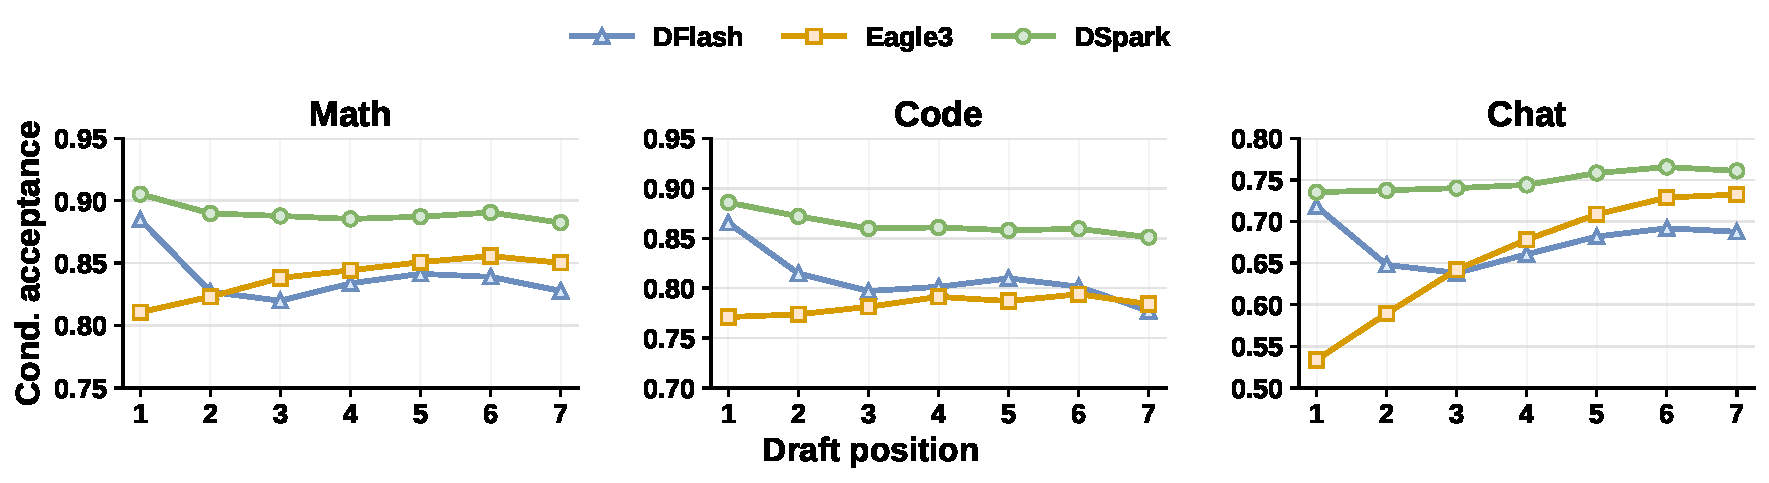
\includegraphics[width=0.95\linewidth]{figs/position_cond_accept.pdf}   
    \caption{\textbf{Position-wise conditional acceptance.} We report the empirical conditional acceptance rate for each draft position, averaged across benchmarks within each domain using the Qwen3-4B target model. Unlike standard prefix survival, this metric isolates the baseline predictive quality at position $k$ by removing the penalty of previous rejections. Notice that the autoregressive drafter (Eagle3) remains stable or trends upward, while the parallel drafter (DFlash) suffers suffix decay.}   
    \label{fig:position_cond_accept}   
\end{figure}   

\autoref{tab:main_exp} presents a counter-intuitive observation: the parallel drafter (DFlash) and the semi-autoregressive drafter (DSpark) often yield longer accepted lengths than the fully autoregressive drafter (Eagle3).
This finding contrasts with the standard expectation that step-by-step autoregression produces higher-quality sequences than parallel models~\citep{ren2020study, israel2026accelerating,zheng2025maskeddiffusionmodelssecretly}.

To analyze this behavior, we examine performance beyond the macro-level accepted length. Using the Qwen3-4B target model and the benchmark sets described in \autoref{sec:exp_setup}, we introduce \textit{position-wise conditional acceptance} tracked during actual speculative decoding rollouts. Specifically, for a given draft position $k$, the evaluation denominator counts only the instances where the target model successfully verifies and accepts all preceding draft tokens from $1$ to $k-1$. The metric then calculates the proportion of these valid instances where the token at position $k$ is also accepted. This approach ensures that the evaluation of position $k$ is not penalized by earlier prefix errors, revealing the underlying predictive quality at each specific step. \autoref{fig:position_cond_accept} details these measurements, demonstrating clear behavioral differences across the architectures.


\paragraph{The Capacity Advantage at Position 1.} 
At the first draft position, both architectures predict the next token based solely on the target context. The performance divergence here stems strictly from architectural capacity: autoregressive models like Eagle3 are constrained to shallow networks due to their $O(\gamma)$ latency, whereas $O(1)$ parallel drafters can afford much deeper networks. This structural gap yields a substantial accuracy margin at position 1, with DFlash starting noticeably higher than Eagle3 (e.g., 0.88 vs.\ 0.81 on Math, and 0.72 vs.\ 0.53 on Chat). Because speculative decoding operates as a strict prefix-matching survival process, the first token carries the highest leverage—a rejection here immediately invalidates the entire block. Consequently, this initial capacity advantage disproportionately boosts the final accepted length, explaining why parallel drafters ultimately outperform autoregressive ones globally despite rapid acceptance decay at later positions.

\paragraph{The Limitation of Independence at Later Positions.} 
Examining the tail of the curves (positions 2 through 7) exposes the inherent limitation of independent parallel generation. As earlier tokens lock in a specific semantic path, subsequent tokens naturally become more predictable. Autoregressive models like Eagle3 effectively leverage this conditional certainty, maintaining or even increasing conditional acceptance deeper into the block (e.g., from 0.53 to 0.74 on Chat). In contrast, DFlash suffers from rapid acceptance decay, dropping from 0.87 to 0.78 on Code and 0.72 to 0.63 on Chat. Because each parallel position marginalizes over all possible prior tokens rather than conditioning on an exact sampled prefix, the model frequently proposes inconsistent suffix combinations—a mode known as multi-modal collision~\citep{gu2018nonautoregressive,stern2018blockwiseparalleldecodingdeep}.

\paragraph{Mitigating Suffix Decay with Semi-Autoregression.}
The preceding analysis highlights a clear architectural objective: combining the high capacity of a parallel backbone for the initial token with the dependency modeling of an autoregressive model for subsequent tokens. This directly motivates DSpark's semi-autoregressive design. As shown in \autoref{fig:position_cond_accept}, DSpark inherits the high initial acceptance of the deep parallel drafter (e.g., starting at 0.93 on Math). Simultaneously, its lightweight sequential head mitigates the rapid acceptance decay typical of parallel generation. By resolving this trade-off, DSpark maintains a high and stable conditional acceptance rate throughout the entire draft block.

\subsubsection{A Little Autoregression Goes a Long Way}  
\label{sec:exp_depth_width}  

Building on the insights from \autoref{sec:parallel_vs_ar_analysis}, we explore the architectural design space of DSpark along two dimensions: drafter depth (number of transformer layers) and proposal length (block size $\gamma$).  
Unless otherwise stated, all experiments in this section use Qwen3-4B as the target model and follow the evaluation protocol detailed in \autoref{sec:exp_setup}.

\begin{figure}[t]
    \centering
    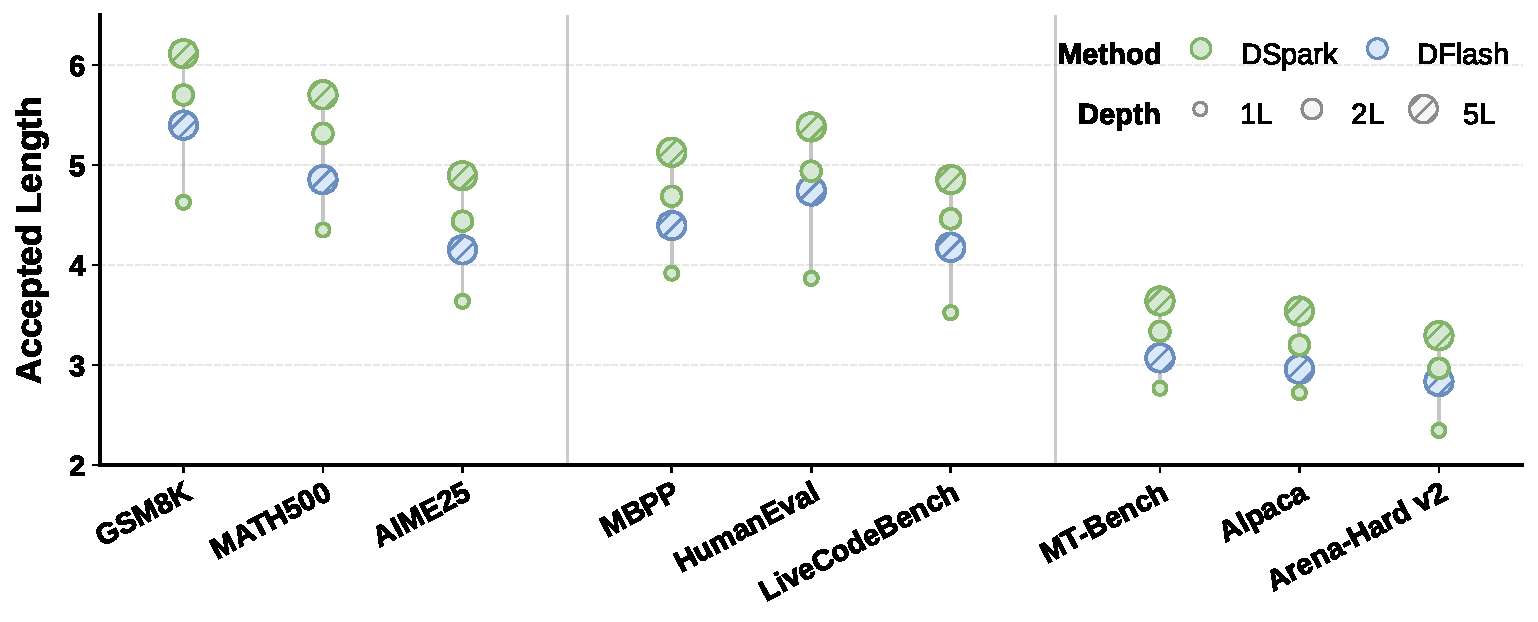
\includegraphics[width=0.9\linewidth]{figs/layer_comparison.pdf}
    \caption{\textbf{Effect of drafter depth.} With proposal length fixed, DSpark's performance improves as drafter layers are added. Notably, a shallow 2-layer DSpark outperforms a deeper 5-layer DFlash baseline, highlighting the parameter efficiency of sequential modeling.}
    \label{fig:layer_comparison}
\end{figure}

\begin{figure}[t]
    \centering
    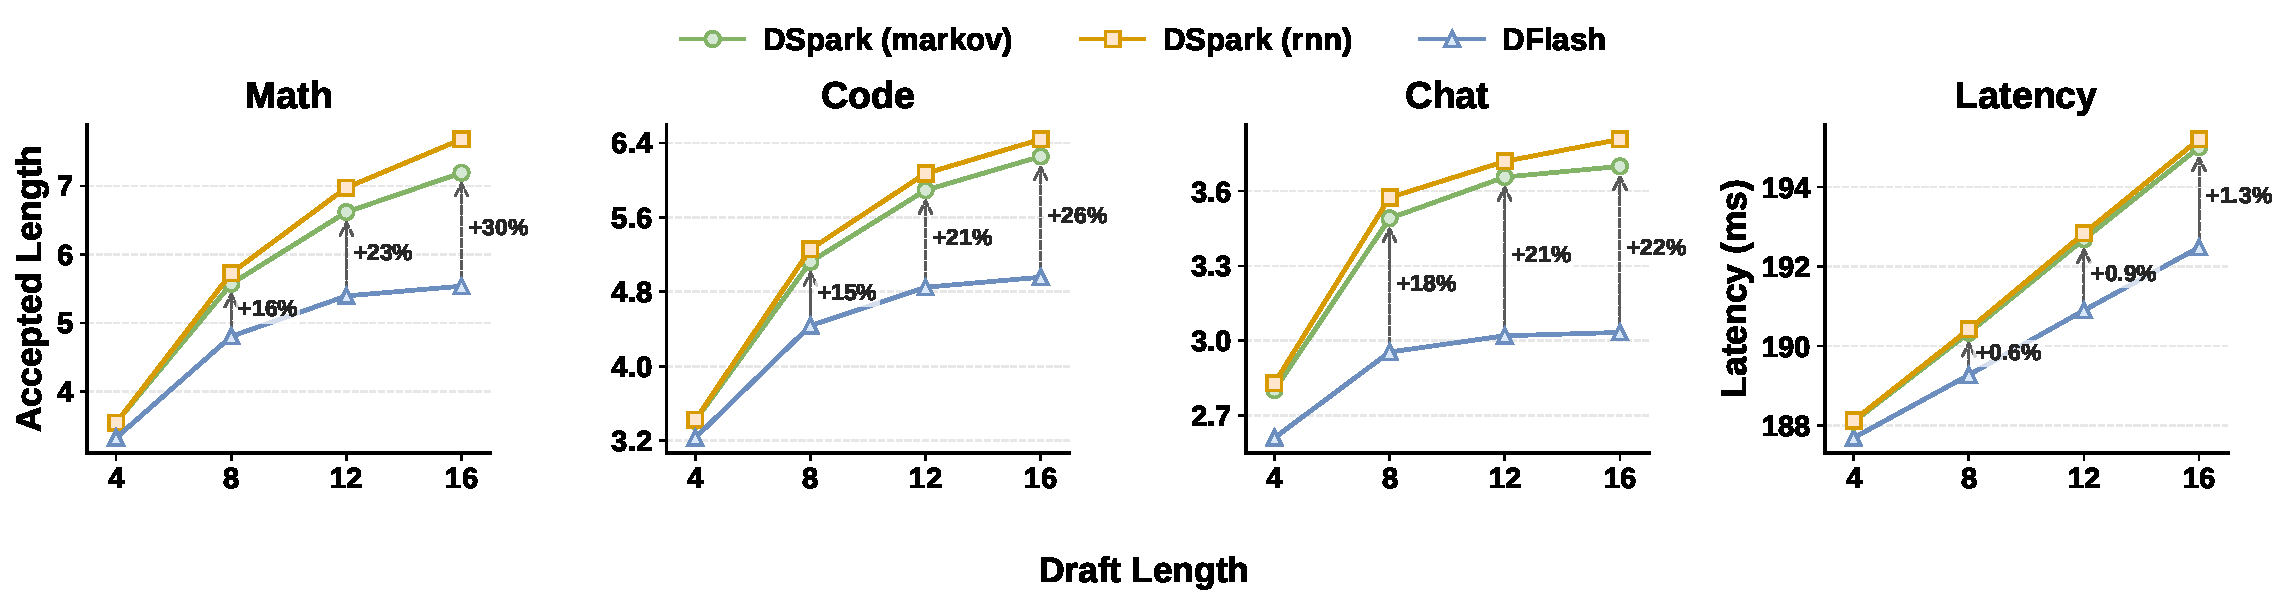
\includegraphics[width=0.95\linewidth]{figs/block_size_comparison.pdf}
    \caption{\textbf{Effect of proposal length and latency overhead.} DSpark consistently outperforms DFlash across various block sizes (left three panels). The rightmost panel demonstrates that the sequential head introduces minimal latency overhead during serving.}
    \label{fig:length_comparison}
\end{figure}

\paragraph{Drafter Depth.}  
Increasing the number of transformer layers naturally expands a draft model's predictive capacity. To isolate this effect, we fix the block size to 7 and vary the number of DSpark layers from 1 to 5, comparing it against a 5-layer DFlash baseline. 
\autoref{fig:layer_comparison} aggregates the accepted lengths across the math, code, and chat domains.  
As expected, DSpark's performance improves monotonically with depth, with the steepest marginal gain occurring from one to two layers.  
Notably, a 2-layer DSpark outperforms the 5-layer DFlash baseline across all domains. This demonstrates that injecting local auto-regression via a lightweight sequential head offers a highly favorable accuracy-parameter trade-off, achieving better sequence coherence than simply stacking deeper parallel layers.

\paragraph{Proposal Length.}
Next, we fix the drafter depth to 5 layers and scale the draft length (proposal length $\gamma$ plus one anchor token) across $\{4, 8, 12, 16\}$ to evaluate performance on longer draft blocks. For DSpark, we evaluate both the default Markov head and the RNN head. The first three panels of \autoref{fig:length_comparison} show that DSpark consistently outperforms DFlash at every proposal length. More importantly, the performance gap steadily widens as $\gamma$ increases. Because pure parallel generation (DFlash) suffers from rapid acceptance decay (\autoref{fig:position_cond_accept}), its marginal utility diminishes for long blocks. DSpark mitigates this decay, causing its relative gain over DFlash to grow. For instance, at $\gamma=7$, DSpark improves the accepted length by 16\% on math, 15\% on code, and 18\% on chat; at $\gamma=15$, these gains expand to 30\%, 26\%, and 22\%, respectively. Also, RNN head provides only marginal additional gains over the Markov head, mainly at longer proposal lengths. Given its higher implementation complexity and less favorable deployment properties, we use the Markov head as the default.

\paragraph{Latency Overhead.}  
We quantify the overhead of the sequential generation loop in DSpark. The rightmost panel of \autoref{fig:length_comparison} reports the per-round engine latency—comprising one target verification pass, the parallel draft block forward, and the serial sampling loop—measured at a batch size of 128. To prevent sequence-length bias, the reported latency represents the arithmetic mean across varying context lengths ($\{512, 1024, 2048, 4096\}~ \text{tokens}$). 
Since the target model dominates the verification compute time at this batch size, the sequential block's latency overhead is negligible. Consequently, scaling the draft length from 4 to 16 adds a marginal 0.2\% to 1.3\% to the full-round latency over the DFlash baseline, despite delivering up to a 30\% improvement in accepted length.  

\subsubsection{Verify Smarter, Not Longer: The Role of Confidence Head}
\label{sec:exp_confidence}

While DSpark sustains high acceptance over long draft blocks, verifying the entire proposal remains inefficient~\citep{huang2024specdec++,hu2026echo}. Due to the inherent domain variance noted in \autoref{sec:exp_main_results}, trailing tokens in open-ended chat still face high rejection risks, making blind verification a waste of target compute. To evaluate whether the confidence head can effectively prune these unpromising suffixes, we conduct an offline threshold sweep using Qwen3-4B. We validate the estimator in isolation here, reserving the hardware-aware prefix scheduler (\autoref{sec:scheduler}) for live production evaluation in \autoref{sec:real_world_deployment}.

\begin{figure}[t]
    \centering
    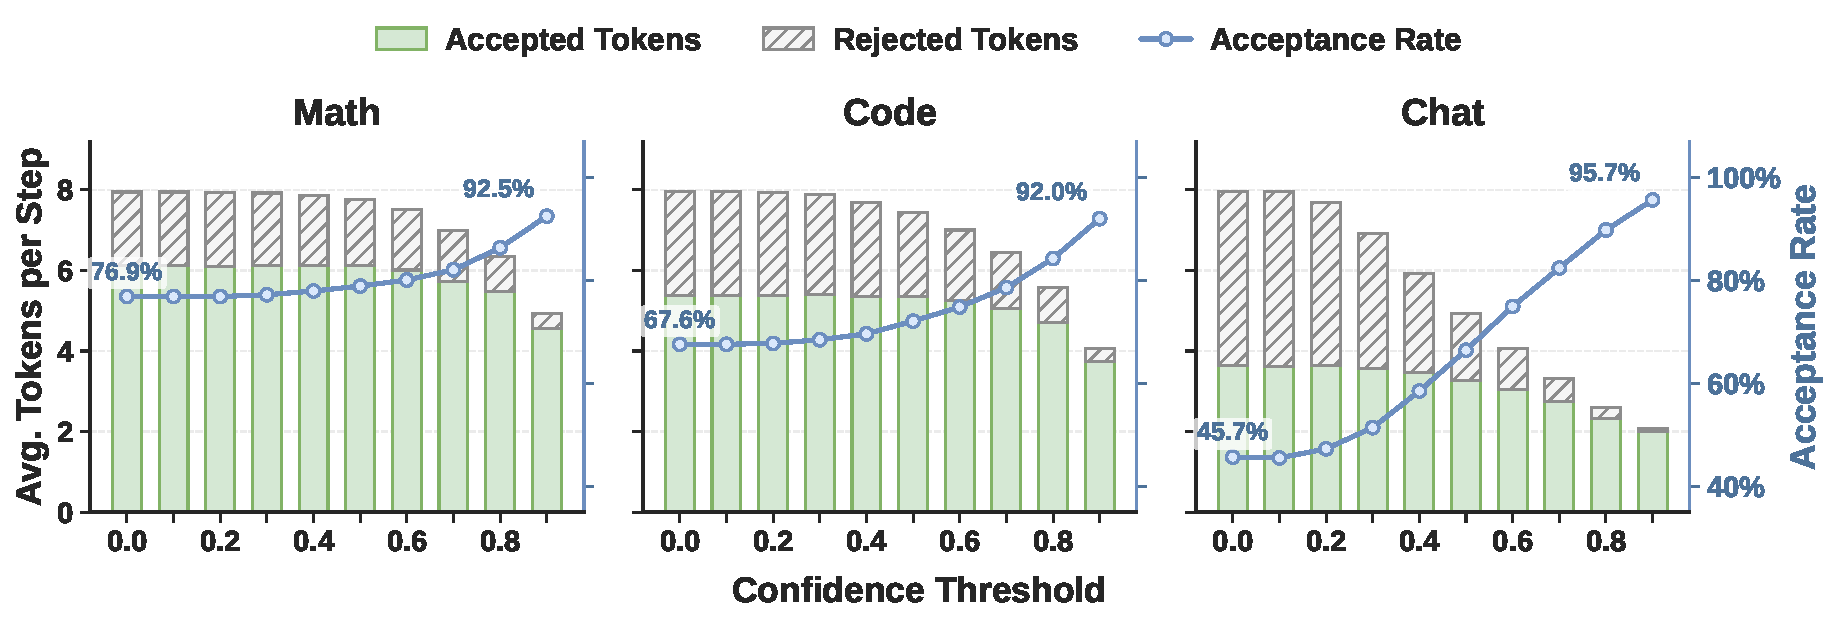
\includegraphics[width=0.95\linewidth]{figs/confidence_threshold_sweep.pdf}
    \caption{\textbf{Confidence threshold sweep.} A threshold of 0 corresponds to standard fixed-length verification. As the threshold increases, the overall acceptance rate steadily rises because the confidence head effectively prunes tokens that would ultimately be rejected (hashed bars).}
    \label{fig:confidence_head_sweep}
\end{figure}

\begin{figure}[t]
    \centering
    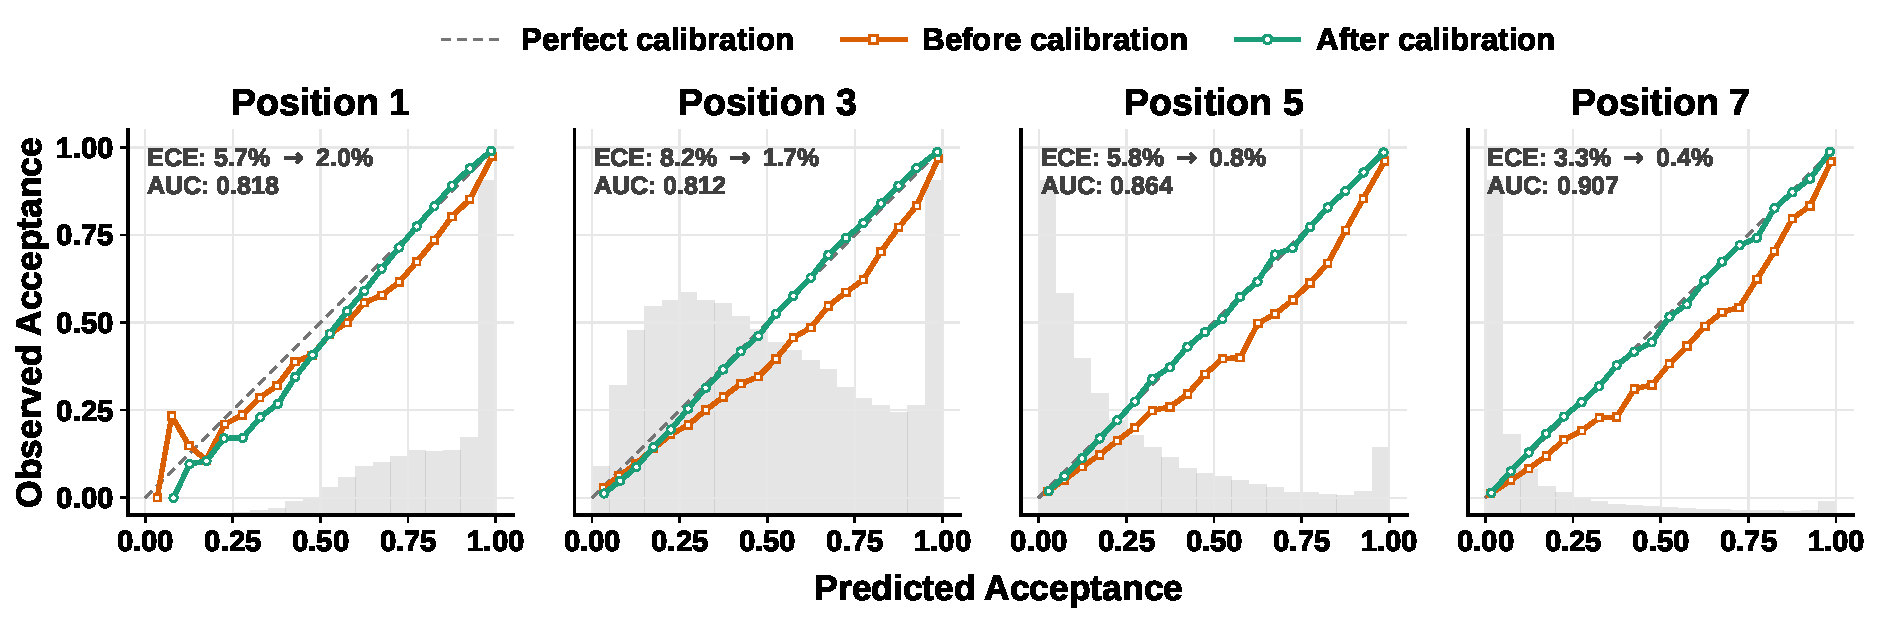
\includegraphics[width=0.95\linewidth]{figs/calibration_alpaca.pdf}
    \caption{\textbf{The Reliability Diagram on Alpaca Dataset.} While the raw confidence estimator achieves strong discrimination, its predictions are inherently overconfident. Applying post-hoc calibration helps to align the prefix survival probabilities with empirical acceptance rates. The shaded background histogram represents the frequency distribution of sample counts across different confidence bins.}
    \label{fig:confidence_head_calibration}
\end{figure}

\paragraph{Diagnostic: Static Threshold Sweep.} 
\autoref{fig:confidence_head_sweep} plots the average tokens per step (bars) and the overall acceptance rate (line) across confidence thresholds. As the threshold increases, the acceptance rate steadily rises because the estimator filters out tokens that would ultimately be rejected (hashed bars). 
This suggests that the confidence head can identify lower-value suffix tokens and this pruning is most pronounced on chat workloads, where higher-entropy token distributions limit the efficiency of fixed-length verification. In the Chat subplot, raising the threshold significantly reduces rejected tokens, increasing the acceptance rate from 45.7\% to 95.7\%. In contrast, structured tasks (Math and Code) experience milder pruning and retain more draft tokens, with acceptance rates rising from 76.9\% to 92.5\% and 67.6\% to 92.0\%, respectively. 
% This confirms that the estimator naturally targets domains where compute waste is highest.

\paragraph{From Static Thresholds to Calibrated Scheduling.}
While useful for diagnostics, a static threshold is sub-optimal in dynamic serving environments because it ignores system load: verifying low-confidence tokens incurs minimal opportunity cost under low concurrency, but wastes critical batch capacity under high concurrency. This load dependency motivates the hardware-aware prefix scheduler. As formulated in \autoref{sec:confidence}, maximizing system-level throughput requires the confidence model to exhibit both strong predictive discrimination and precise calibration to accurately estimate cumulative survival probabilities. The reliability diagram~(\autoref{fig:confidence_head_calibration}) demonstrates that while the raw model achieves strong discrimination (ROC-AUC~\citep{hanley1982meaning} ranging from 0.81 to 0.90), it is overly confident (ECE 3\%--8\%). Applying post-hoc STS~(\autoref{sec:conf_head}) mitigates this overconfidence, reducing the average ECE to $\sim$1\% and yielding reliable survival estimates.